\chapter{Yet another tool: XCorex }\label{ch:3}

\epigraph{Programming today is a race between software engineers striving to
build bigger and better idiot-proof programs, and the Universe trying to produce
bigger and better idiots. So far, the Universe is winning.}{Rich Cook}

	For the problems presented in chapter \ref{ch:2.2} I have implemented a tool
that defines a meta-metamodel as described in chapter \ref{ch:2.1.1} which will
allow you to describe the metamodel for the tool you want to implement and it will generate 
a model based on the data you provided. In order to evaluate the application I
have also reimplemented a front-end tool called InsiderView \cite{tools:iPlasma}
which allows you to integrate different metrics based on the meta-metamodel from 
CodePro.
	During the implementation phase there were a number of different ideas
that were proposed and/or implemented in order to fully understand the
limitations of annotation processing and code generation in java and also to
provide the most general solution which can be used by as many users as
possible.

\section{XCorex}

\subsection{Solution Overview}
	 
\begin{figure}
\centering
\scalebox{0.5}{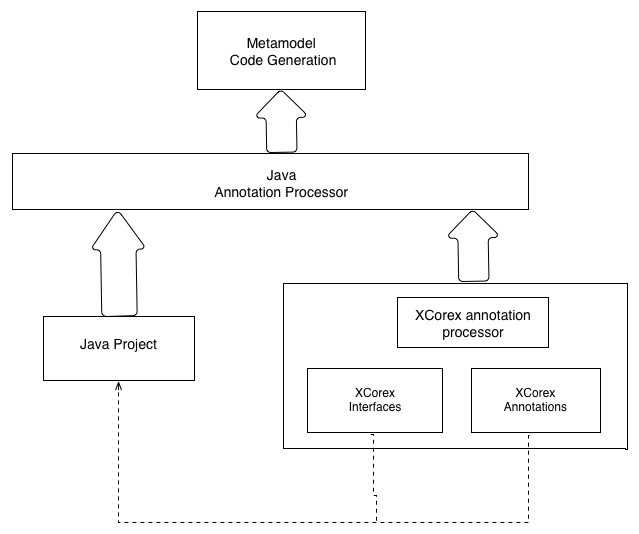
\includegraphics{img/solution/XCorexSystem.png}}
\caption{XCorex System overview}
\label{fig:XCorexSystem}
\end{figure}

	Figure \ref{fig:XCorexSystem} represent the  general system architecture. 
As it can be seen there are three main components that describe the XCorex
system:
	\begin{itemize}
	  \item Annotation Component
	  \item Interface  Component
	  \item Annotation Processor
	\end{itemize}
	The XCore annotation component represent the implementation of the
meta-metamodel as presented in chapter \ref{ch:2.1.1} and provides the necessary
metadata to describe the metamodel which is implemented by the client. 
	The XCorex interface component helps the client in describing the necessary
elements for the model of the application and also enforces a type safe environment.
	The above two components describe the semantics of our system which is enforced 
by the annotation processor. The processor is, if you will, the brain of system
which analysis the metadata provided by client with the help of the two
components and generates the appropriate model. 

\subsection{Implementation Details}

\subsubsection{Annotation Component}
	
	This component describes two 

\subsubsection{Interface Component}

\subsubsection{Annotation Processor}


\section {XCorexView}

\subsection {InsiderView overview}

\subsection {What has changed}

	